\documentclass[12pt, a4paper]{exam}
\usepackage{graphicx}
\usepackage[left=0.8in, top=0.7in, total={6.2in,8in}]{geometry}
\usepackage[normalem]{ulem}
\usepackage{listings}
\usepackage{xcolor}
\definecolor{codegreen}{rgb}{0,0.6,0}
\definecolor{codegray}{rgb}{0.5,0.5,0.5}
\definecolor{codepurple}{rgb}{0.58,0,0.82}
\definecolor{backcolour}{rgb}{1,1,1}
\lstdefinestyle{mystyle}{
    backgroundcolor=\color{backcolour},   
    commentstyle=\color{codegreen},
    keywordstyle=\color{magenta},
    numberstyle=\tiny\color{codegray},
    stringstyle=\color{codepurple},
    basicstyle=\ttfamily\footnotesize,
    breakatwhitespace=false,         
    breaklines=true,                 
    captionpos=b,                    
    keepspaces=true,                 
    numbers=left,                    
    numbersep=5pt,                  
    showspaces=false,                
    showstringspaces=false,
    showtabs=false,                  
    tabsize=2
}

\lstset{style=mystyle}
\renewcommand\ULthickness{1.0pt}   %%---> For changing thickness of underline
\setlength\ULdepth{1.3ex}%\maxdimen ---> For changing depth of underline

\begin{document}
	%\thispagestyle{empty}
	\noindent
	\begin{minipage}[l]{0.1\textwidth}
		\noindent
		
\includegraphics[width=2.4\textwidth]{logo.png}
	\end{minipage}
	\hfill

\begin{minipage}[c]{0.8\textwidth}
	\begin{center}
		{\large Universidad La Salle \par
		\small Ingeniería de Sofware	\par
		\large Fundamentos de Lenguajes de Programación	\par
\small Karlo Pacha Curimayhua \par
\small Fecha: Octubre 25, 2022} \par
	\end{center}
\end{minipage}
\par
\vspace{0.2in}
\noindent
\par 
\vspace{0.15in}
\noindent
\centering { \small \bfseries Práctica 13 } \par
\centering { \small \ Ejercicios }


%q1
\begin{questions}
	\pointsdroppedatright
	\question Investigue el concepto de first class en Javascript y muestre una pequeña defición seguida ejemplos. (2 puntos)
	\begin{parts}
		\part Son funciones que son tratadas como cualquier otra variable; estas puedes ser pasadas como argumento a otras funciones, puede ser retornada por otra función y puede ser asignada a una variable.
	\end{parts}
\vspace{0.2in}

\lstinputlisting[language=Octave]{1.js}

%q2
\pointsdroppedatright
	\question Describa la diferencia entre Currying and Partial Application. Incluya ejemplos. (2 puntos)
	\begin{parts}
		\part Currying: Una función que toma una función con múltiples parámetros como entrada y devuelve una función con exactamente un parámetro.
		\part Partial Application: El proceso de aplicar una función a algunos de sus argumentos. La función aplicada parcialmente se devuelve para su uso posterior. 
		\vspace{0.05in}
	\end{parts}
\vspace{0.2in}

\lstinputlisting[language=Octave]{2.js}

%q3
\pointsdroppedatright
	\question Implemente una función que calcule el volumen de un cilindro. Incluya la versión normal y una aplicando Currying. (2 puntos)
	\lstinputlisting[language=Octave]{3.js}

	\begin{figure}[h]
		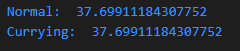
\includegraphics[width=8cm]{3.png}
	\end{figure}
\vspace{0.2in}

%q4
\pointsdroppedatright
	\question Cree una función joinWords que una varios parametros de tipo string. (3 puntos)
	\lstinputlisting[language=Octave]{4.js}

	\begin{figure}[h]
		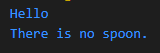
\includegraphics[width=8cm]{4.png}
	\end{figure}
\vspace{0.2in}

%q5
\pointsdroppedatright
	\question Implemente una función delayInvoc que en cada invocación incremente la variable total con el valor enviado como parametro. (3 puntos)
	\lstinputlisting[language=Octave]{5.js}

	\begin{figure}[h]
		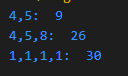
\includegraphics[width=8cm]{5.png}
	\end{figure}
\vspace{0.2in}

%q6
\pointsdroppedatright
	\question Implemente una función curry que tome como argumento cualquier función f y retorne la versión curried de f. (4 puntos)
	\lstinputlisting[language=Octave]{6.js}

	\begin{figure}[h]
		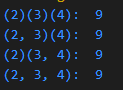
\includegraphics[width=8cm]{6.png}
	\end{figure}
\vspace{0.2in}

\large GitHub: 
\small https://github.com/KEPCU/FundamentalsOfProgrammingLanguages/tree/master/js/practice13
\end{document}